\section{Earlier natural-image protocols and diagnostics}
\label{app:natural-details}
Natural-image experiments test whether direction selection has observable task consequences beyond the controlled construction. They reveal substantial objective improvement without substantial class-readability gains, and a local risk-direction effect with limited coverage and persistence. On CIFAR-10~\cite{krizhevsky2009learning}, we use grayscale input, 64 $11\times11$ valid convolutional filters, squaring, GAP, and an eight-dimensional head. Unsupervised pretraining starts from scratch without downstream labels. The training split is 45,000/5,000, and the standard 10,000-image test set is reserved for the fixed final-budget comparison. Augmentations are reflected crops, horizontal flips, contrast changes, and additive noise. Classification uses unregularized affine OLS on one-hot labels, evaluating encoder and projection separately. Validation MSE is a finite-sample task risk, not the theorem's population risk. Supervised references and the label-conditioned intervention below are distinguished from pretraining.

\subsection{Layerwise rates do not establish a speed-independent gain}
Five paired seeds and three ratios run for 4,000 updates at batch size 256, approximately 22.8 training-set passes. Encoder test accuracy is $36.48\%$, $36.45\%$, and $36.52\%$ for $r=0.1,1,10$; projection accuracy is $23.39\%$, $23.50\%$, and $23.81\%$. The fixed-budget projection difference is approximately $0.43$ percentage points before rounding the group means. At common calibration energy $\ell=2$, however, the corresponding validation difference is approximately $+0.11$ points with a five-seed descriptive bootstrap interval $[-0.42,+0.54]$. Other common-energy intervals also cross zero. Energy is measured on a fixed unlabeled calibration set and its first crossing is checked every ten updates; it is a proxy with recorded overshoot, not an exact population progress variable. The results do not establish either a stable speed-independent benefit or its absence.

\subsection{More capacity mostly improves the initial features}
Development diagnostics use seeds 0, 1, and 12, three architectures, and two supervised references, for 33 runs of 4,000 updates. These runs use validation labels only for evaluation, never the test set. Table~\ref{tab:capacity} separates initial performance from learned improvement.

\begin{table}[t]
\centering\small
\caption{Validation OLS accuracy (\%) for capacity diagnostics, $r=1$; means over three development seeds. Each cell shows initialization $\to$ 4,000 updates.}
\label{tab:capacity}
\setlength{\tabcolsep}{4pt}
\begin{tabular}{lrr}
\toprule
Architecture&Encoder&Projection\\\midrule
$C=64,K=8$&$36.31\to36.04$&$23.49\to23.71$\\
$C=256,K=8$&$43.04\to43.04$&$23.66\to23.65$\\
$C=64,K=32$&$36.31\to36.23$&$32.05\to32.14$\\
\bottomrule
\end{tabular}
\end{table}

Width and projection dimension improve absolute readability, but their gains largely exist at random initialization. Supervised training of the original model reaches encoder OLS accuracy $40.07\%$ through the encoder path and projection OLS accuracy $38.69\%$ through the joint projection path. Thus $24\%$ is not an expressivity ceiling for eight-dimensional outputs. The supervised references use Adam and prescribed gradient clipping, unlike unsupervised SGD, and are attainable references rather than matched optimization or capacity upper bounds.

The wide model has a small exploratory ratio signal: $r=10$ minus $r=0.1$ projection accuracy is positive for all three development seeds at $\ell=1$ and $2$, with means near $+0.20$ and $+0.19$ points. Multiple inspected sections, few development seeds, and inconsistent MSE signs at some sections prevent a stable intervention claim. Some $K=32$ energy sections are missing; we retain those missing cases rather than treating available pairs as a complete experiment.

\subsection{A fixed encoder admits a much better eight-dimensional head}
We freeze the original $r=1$ encoder at initialization and update 4,000 for each development seed: six source states, with only three independent seeds. Each state compares the original head, full encoder OLS, an optimal rank-8 affine least-squares fit, and a supervised head trained with cross-entropy (CE). The rank-8 solution uses training labels only. Its affine intercept is absorbed into the final decoder, leaving the projection itself linear. CE training updates only the projection and classifier; kernels are checked for exact equality before and after training.

\begin{table}[t]
\centering\small
\caption{Same frozen encoder, different heads. Validation accuracy (\%), three paired development seeds per source state.}
\label{tab:frozen}
\setlength{\tabcolsep}{3pt}
\begin{tabular}{lrr}
\toprule
Readout&Initial&Trained\\\midrule
Full encoder OLS&36.31&36.04\\
Original head + OLS&23.49&23.71\\
Rank-8 least squares&35.75&35.59\\
CE-trained head + OLS&30.89&28.49\\
CE-trained classifier&30.83&27.73\\
\bottomrule
\end{tabular}
\end{table}

For the trained encoder, rank-8 fitting improves accuracy over the original head by approximately $11.88$ points, remaining only $0.45$ points below full encoder OLS. Its validation one-hot MSE is $0.08147432$, compared with $0.08631537$ for the original head and $0.08141745$ for the full encoder. It removes $98.84\%$ of this particular MSE gap; this is not a percentage of all semantic information. A better compressed choice exists without any encoder change.

Crucially, almost the same gap is already present at initialization. These data do not show that pretraining created a large new semantic loss. The CE-trained head improves over the source head but falls short of rank-8 fitting even on training accuracy ($28.71\%$ versus $36.59\%$). The gap is therefore not solely a validation overfitting effect, but CE versus square loss, augmented versus clean inputs, scaling, clipping, and budget are confounded; factorized optimization alone is not identified as its cause.

Ten-class centered one-hot targets have at most nine independent directions, so near-recovery by eight coordinates has a direct algebraic context. Reduced-rank fitting is globally optimal for training MSE, not validation accuracy. It establishes available task-dependent compression, not a label-free way to find it or an architecture-specific phenomenon.

\begin{figure}[t]
\centering
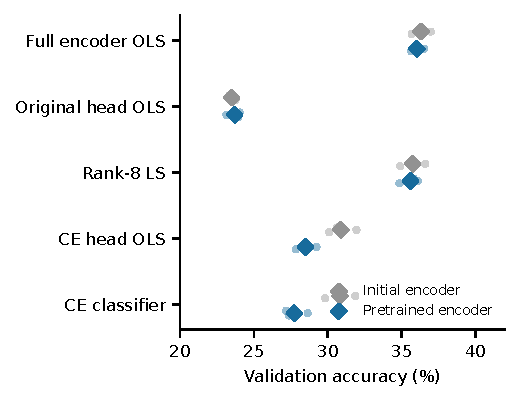
\includegraphics[width=\linewidth]{figures/frozen_heads.pdf}
\caption{Validation accuracy for different readouts of the same fixed encoder. Points are paired development seeds. The large source-head gap exists both before and after pretraining. Rank-8 fitting is supervised.}
\label{fig:frozen}
\end{figure}

\subsection{Objective improvement amplifies existing image statistics}
The architecture reads local second moments: for valid image patches $p_u$ and filter $h_c$, its encoder coordinate is $h_c^\top M(x)h_c$, where $M(x)=|U|^{-1}\sum_u p_up_u^\top$. This makes existing image-energy statistics plausible optimization directions, but does not establish that they are unrelated to classes.

We examine this explanation on the Describable Textures Dataset (DTD), using official partition 1, $64\times64$ grayscale inputs, the same $64/8$ model, and three development seeds (0, 1, 12), with $r=1$ and 2,000 updates. OLS fits use the official training set and evaluation uses the validation set; no test images are evaluated. In the original pilot, the encoder's leading clean-feature variance share rises from $91.93\%$ to $99.46\%$, while the tail variance remains nonzero. A train-fitted predictor using the squared per-image DC offset relative to the training global mean explains approximately $93.4\%$ of the final leading-component variation on validation images. Encoder training accuracy changes from $17.82\%$ to $17.70\%$, and validation accuracy from $8.65\%$ to $8.51\%$. Thus finite-label probe generalization is a limitation, but cannot alone explain the absence of training-set class gains.

Removing each filter's spatial mean at evaluation suppresses the identified DC response without reliably improving the class task. Training a spatially zero-mean model from initialization likewise produces no clear encoder learning gain: validation accuracy changes from $8.78\%$ to $8.56\%$. Its projection validation MSE improves slightly, from $0.02072149$ to $0.02071484$, while accuracy changes from $6.22\%$ to $6.21\%$. The dominant direction now tracks pixel variance, explaining about $84\%$ of final projection PC1 validation variation; this association already exists at initialization. The projection remainder has a small positive signal (accuracy $4.65\%\to4.89\%$), but does not establish improved full-encoder readability. The zero-DC constraint changes the initial function and training dynamics, so the two runs are not matched-function interventions.

Together these observations are consistent with preferential amplification of existing, augmentation-stable second-order statistics, rather than substantial acquisition of class-predictive directions. They do not isolate the objective, augmentation, or architecture as the unique cause. Spectral concentration alone is not evidence of task-information deletion: full-rank unregularized OLS is invariant to invertible feature-coordinate transformations, and the recorded tail variance and numerical rank persist. Conversely, the observed non-scalar feature changes do not by themselves establish task-relevant learning.

\subsection{Local risk reversal exists but has limited persistence}
We directly test two-block competition using the CIFAR $r=1$ checkpoints at updates 0, 1,000, and 4,000 for the same three development seeds. Each state has three paired future streams, giving 27 state--stream combinations, not 27 independent samples. Let $R$ denote validation one-hot MSE after refitting training-set affine OLS. With source mobility $m$, base rate $\eta$, and block training gradients $g_h,g_W$, define
\begin{align}
 A&=\langle\nabla_h R,-\eta m g_h\rangle,\nonumber\\
 B&=\langle\nabla_W R,-\eta m g_W\rangle,\nonumber\\
 \Delta R(r,s)&\approx \frac{2s}{1+r}(A+rB).
 \label{eq:natural-local}
\end{align}
The derivative includes the training decoder's dependence on the features. Unlike the analytic population threshold, this is an empirical, label-conditioned calculation. A positive threshold $r_*=-A/B$ requires opposing block contributions. We compare fixed ratios $0.1,1,10$, overall speed controls $s=0.5,2$ at $r=1$, and eligible brackets $r_*/2,2r_*$. Predictions precede branch evaluation; implementation and eligibility details are in Appendix~\ref{app:natural-direction}.

All 27 combinations pass the recorded finite-difference checks. Only four have eligible positive thresholds: none of nine at initialization, one of nine at update 1,000, and three of nine at update 4,000. All four brackets reverse the observed risk sign as predicted after one update, but only two retain that reversal after five updates and none after twenty (Table~\ref{tab:natural-threshold}). The first-step changes are tiny: available seed-level means within source-state/bracket cells have absolute magnitude $7.49\times10^{-10}$ to $4.71\times10^{-9}$, with no accuracy change. First-step agreement checks the local approximation; it is not by itself evidence of a useful control rule or a mechanism unique to this architecture.

\begin{table}[t]
\centering\small
\caption{CIFAR threshold brackets: observed opposite risk signs that both match the source-state prediction. Coverage is 4/27 state--stream combinations across three development seeds. These are repeated measurements, not independent trials.}
\label{tab:natural-threshold}
\begin{tabular}{lrrr}
\toprule
Branch updates&1&5&20\\\midrule
Successful brackets / eligible&4/4&2/4&0/4\\
\bottomrule
\end{tabular}
\end{table}

A small fixed-ratio effect remains at the late source state: after twenty updates, $r=10$ minus $r=1$ validation MSE is $-3.72\times10^{-8}$, $-2.74\times10^{-7}$, and $-2.41\times10^{-8}$ for seeds 0, 1, and 12, respectively, averaging streams within each seed. This is improvement relative to the baseline branch, not uniform improvement relative to the source: seed 1 still increases its risk. Each seed's stream-mean accuracy change for $r=10$ is zero.

The results establish a local correspondence with two-block direction competition, but not the certified finite-time rebound or a stable natural-image intervention. Beyond the first update, both batches and parameters change. Loss of the source threshold's predictive control therefore does not contradict Equation~\eqref{eq:natural-local}; the present measurements do not separate stochastic-gradient variation from state-dependent changes in the local contributions.
